\documentclass[a4paper]{scrartcl}
\usepackage{amsmath,amssymb,amsthm}
\usepackage{bm}
\usepackage{biblatex}
\usepackage{courier}
\usepackage{float}
\usepackage[colorlinks=true, allcolors = black, urlcolor=cyan]{hyperref}
\usepackage{graphicx}
\usepackage{mathtools}
\usepackage{physics}

\renewcommand{\thesection}{\arabic{section}}
\renewcommand{\thesubsection}{\alph{subsection}}

\title{Assignment 1}
\subtitle{TTK4210 - Advanced Control of Industrial Processes}
\author{Sondre Myrberg \\ \href{mailto:sondrmyr@stud.ntnu.no}{sondrmyr@stud.ntnu.no}}
\date{\today}

\setlength{\parindent}{0pt} % Disable indentation
\mathtoolsset{showonlyrefs} % Only show equation numbers on referenced equations


\begin{document}

\hypersetup{pageanchor=false}
\begin{titlepage}
    \maketitle
    \vfill
    \vfill
    \vfill
    \vfill
    \vfill
    \centering
    
\includegraphics[width=0.8\textwidth]{../ntnu_logo.pdf}
    \vfill
    \vfill
\end{titlepage}
\hypersetup{pageanchor=true}

\section{Installation of K-Spice}
Done, nothing more to report from here.\\

\section{}
\subsection{Startup}
Startup completed and model loaded.\\
\subsection{Simulation}
The model simulates nicely with a maximum speed at about 400.\\
\subsection{Graphs and parameters}
The inital values of the controller \texttt{LIC0001} is shown in \autoref{fig:lic0001_init}.

\begin{figure}[ht!]
	\centering
	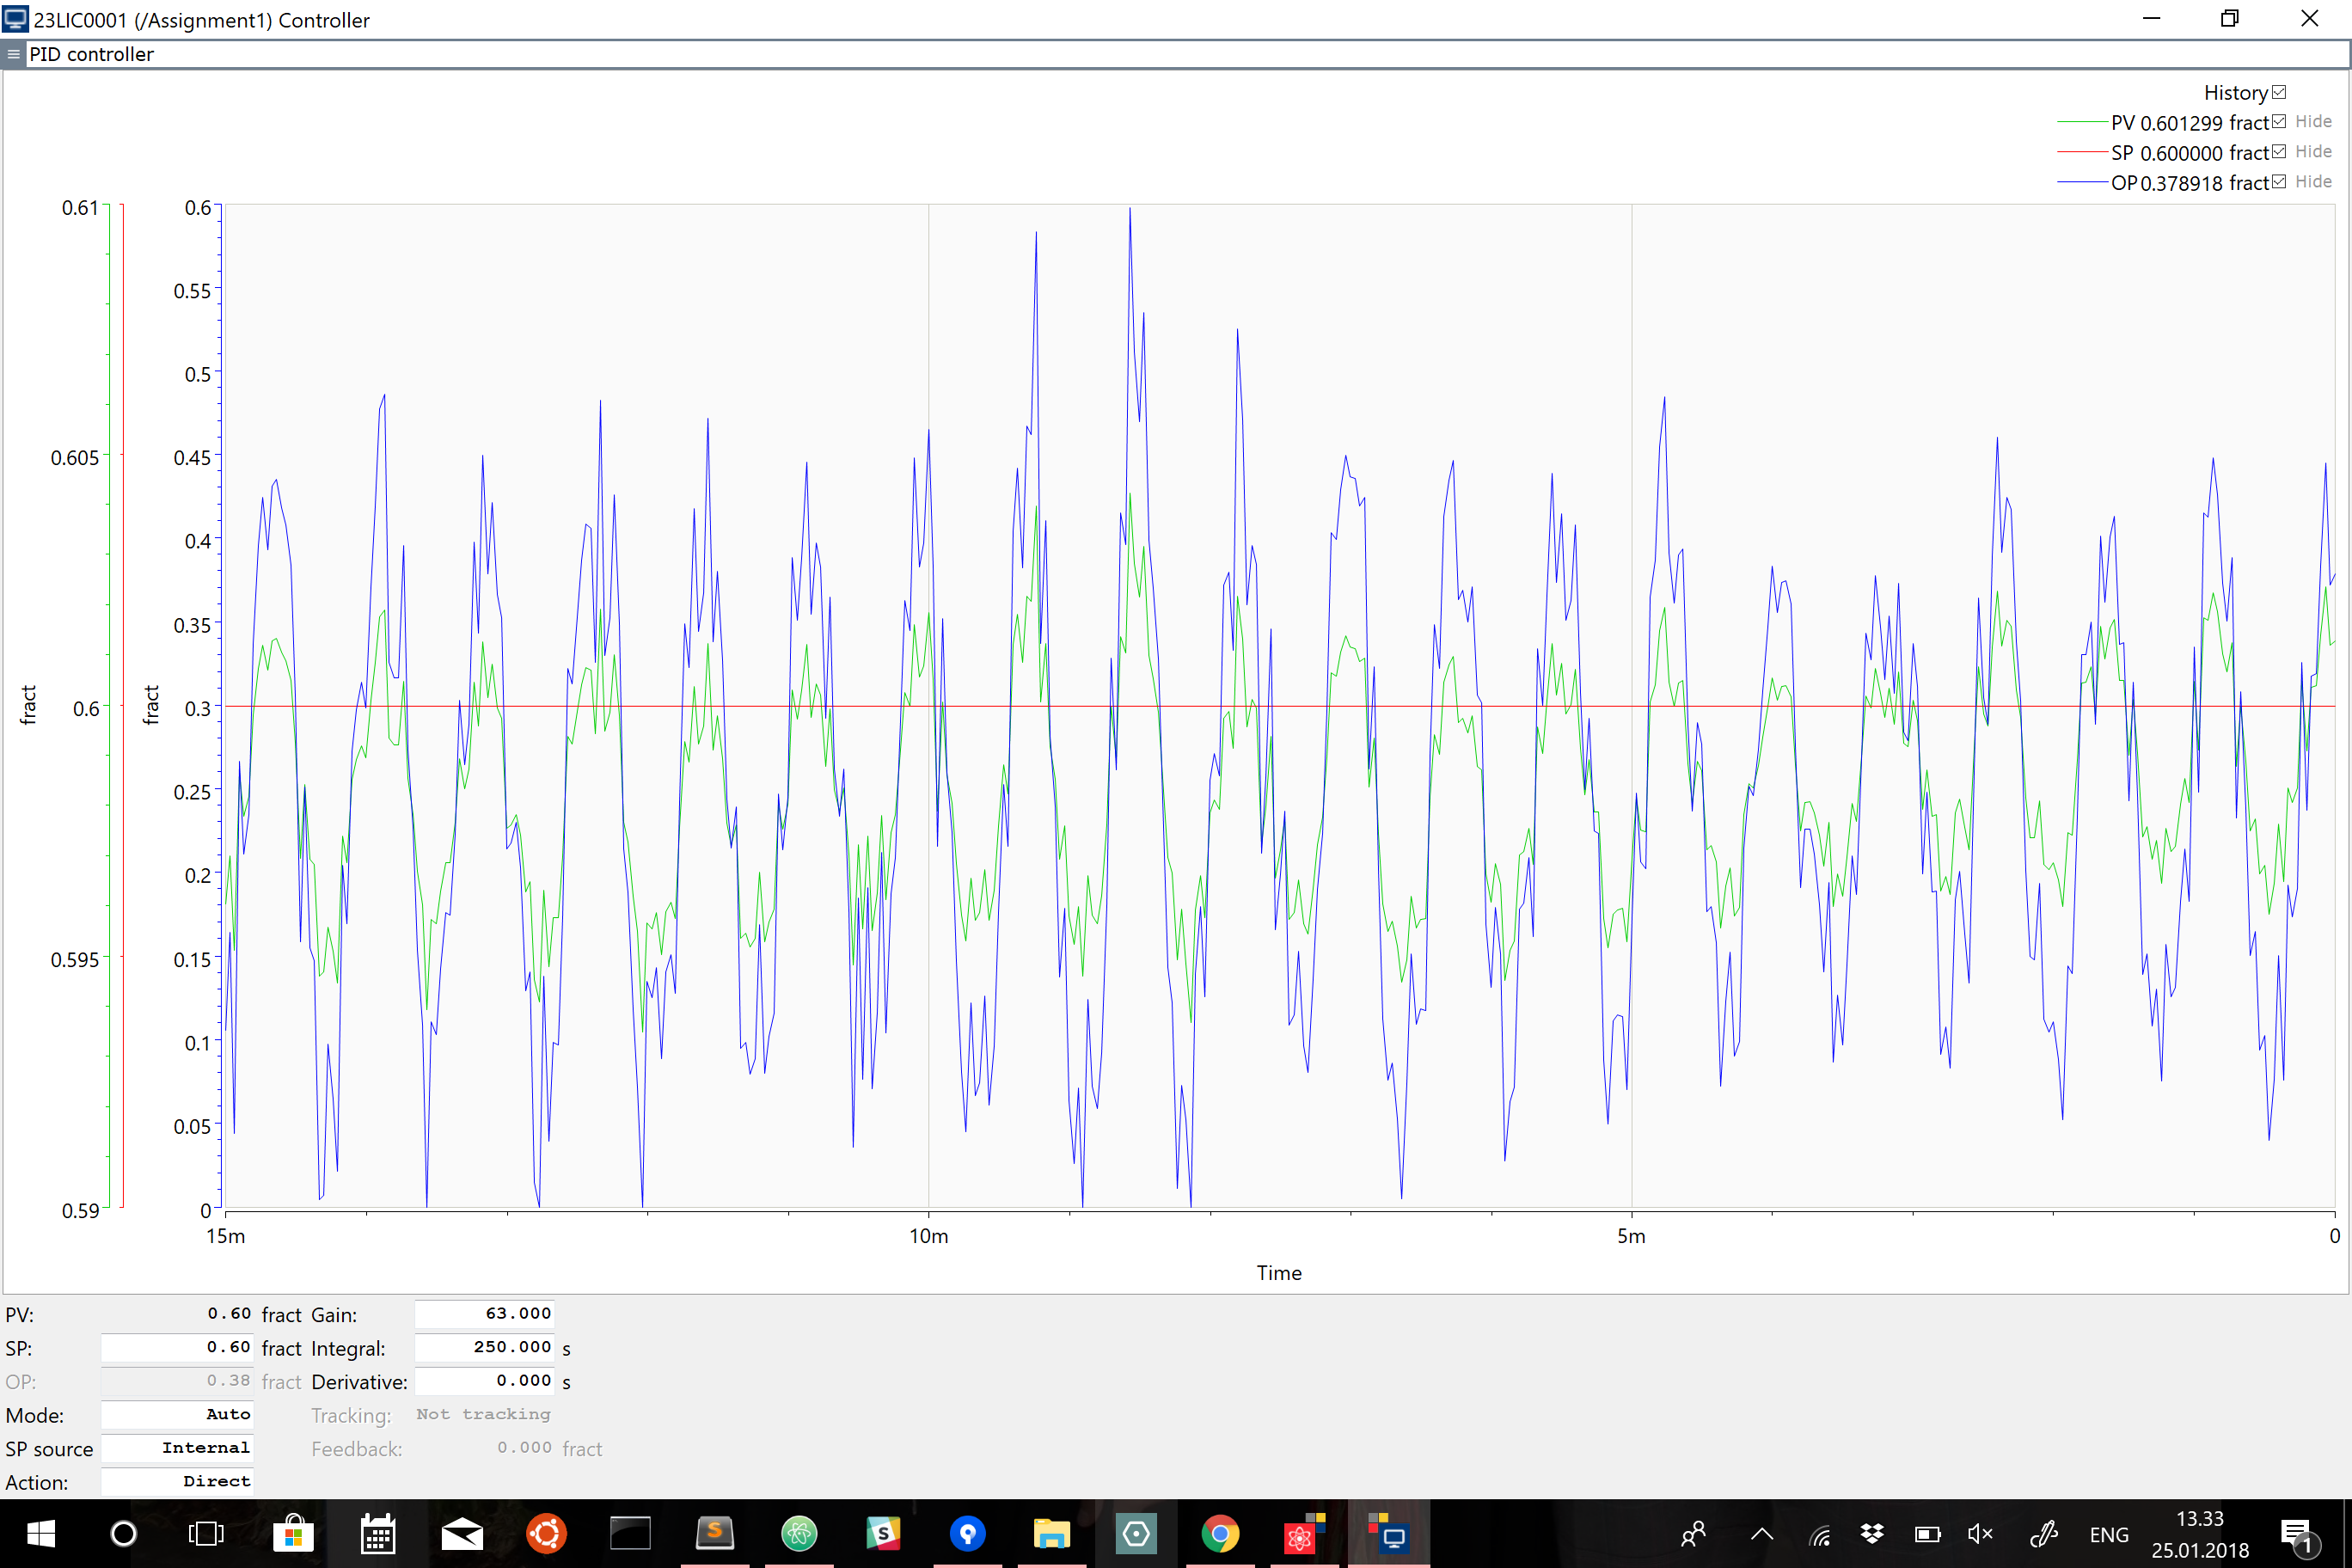
\includegraphics[width=0.7\textwidth]{fig/LIC0001_init.png}
	\caption{Initial values of the controller \texttt{LIC0001}}
	\label{fig:lic0001_init}
\end{figure}

\section{Model survey}
The three main control loops for the 3-phase vessel \texttt{23VA0001} are the control loops for the two levels of fluid and the final loop for the amount of gas inside the vessel.\\

\section{Model simulation and controller tuning}
\subsection{}
In the first controller \texttt{LIC0001} we observe fast dynamics and aggressive controlling, which could be the result of high gain and integral time, which is quite the opposite from the other controller \texttt{LIC0002} which has small gain and short integral time, and corresponding slower dynamics.

\subsection{}
When tuning these controllers a general rule of thumb is tuning the controller with the corresponding fastest dynamics first. This will affect the other controller the least. In this case this is the \texttt{LIC0001} controller.

\subsection{}
Using Skogestad IMC tuning of PID controllers we need to obtain $\Delta u$, $\Delta t$, $\Delta y$, $\theta$ and $\tau_C$ to get our control parameters $K_C$ and $\tau_I$ where $K_C$ is the gain and $\tau_I$ is the integral time. This is given as 
\begin{equation}\label{eq:SIMC}
	\begin{aligned}
		K_C &= \frac{1}{k'} \cdot \frac{1}{\theta + \tau_C}\\
		\tau_I &= \min\{\tau_1 , 4(\tau_C + \theta)\}\\
		k' &= \frac{\Delta y }{\Delta t \Delta u}
	\end{aligned}
\end{equation}
Using the model for a step response integrating model we get no $\tau_1$ and therefore $\tau_I = 4(\tau_C + \theta)$. Further we must chose the tuning parameter $\tau_C$. A rule of thumb for this is for `fast', but more towards oscillating, control we chose $\tau_C = \theta$ and for `slower', but less robust for disturbance, we chose $\tau_C = 3\theta$. Doing an open loop step response on \texttt{LIC0001} we obtain the values
\begin{equation}
	\begin{aligned}
		\Delta u &= 0.1 \quad &&\theta = 20\\
		\Delta y &= 0.114 \quad &&\Delta t = 1048\\
	\end{aligned}
\end{equation}
This yields the following parameters for different $\tau_C$
\begin{center}
	\begin{tabular}{c|c|c}
		$\tau_C$ & $3\theta$ & $\theta$ \\
		\hline
		$K_C$ & $11.49$ & $ 22.98$\\
		$\tau_I$ & $320$ & $160$
	\end{tabular}
\end{center}

For the controller \texttt{LIC0002} we get the values
\begin{center}
	\begin{tabular}{c|c|c}
		$\tau_C$ & $3\theta$ & $\theta$ \\
		\hline
		$K_C$ & $5.99$ & $11.97$\\
		$\tau_I$ & $80$ & $40$
	\end{tabular}
\end{center}
The `fast' controller gets a small oscillation here, but the response with $\tau_C = 3\theta$ gives a fairly good response. All in alle we can conclude that the first controller was too aggressively tuned while the second was too slow. 

\section{Model Control Language (MCL) and data logging}
\subsection{}
When not tuning the controllers we get the responses shown in \autoref{fig:5a1}, \autoref{fig:5a2}, \autoref{fig:5a3} and \autoref{fig:5a4} in \autoref{sec:plots}.

\subsection{}

When the controllers are tuned with the paramters from above we get the responses shown in \autoref{fig:5b1}, \autoref{fig:5b2}, \autoref{fig:5b3} and \autoref{fig:5b4} in \autoref{sec:plots}.


\section{Model survey}
\subsection{}
The component \texttt{ASC0001} is an Anti Surge Controller that protects the compressor from surge. This is critical for the compressor to function properly.
\subsection{}
The \texttt{23HX0001} is a cooler. This component cools the gas that is fed back to the tank in one of the main control loops and the gas that is released. As we need to cool both the air released and the air fed back we place this before the feed back loop, so that we don't need two coolers.
\subsection{}
The component \texttt{PSV0001} is a safety valve to ensure that the pressure in the vessel isn't getting too high and blows up.

\clearpage
\appendix
\section{Plots}\label{sec:plots}
\begin{figure}[ht!]
	\centering
	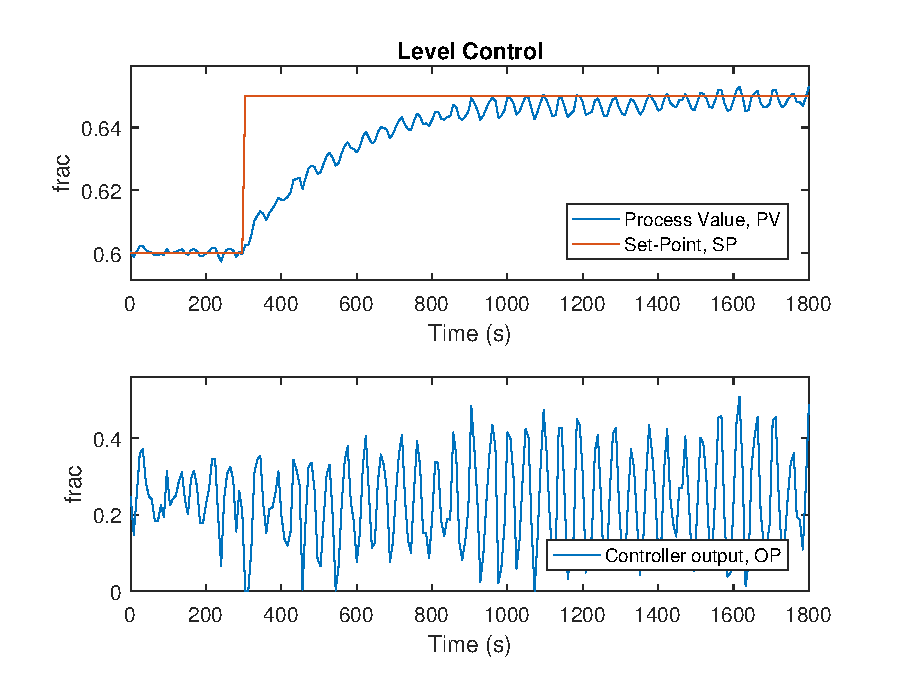
\includegraphics[width=0.7\textwidth]{fig/untuned/LIC0001_step1_untuned.eps}
	\caption{Response in \texttt{LIC0001} with step in the controller \texttt{LIC0001}}
	\label{fig:5a1}
\end{figure}
\begin{figure}[ht!]
	\centering
	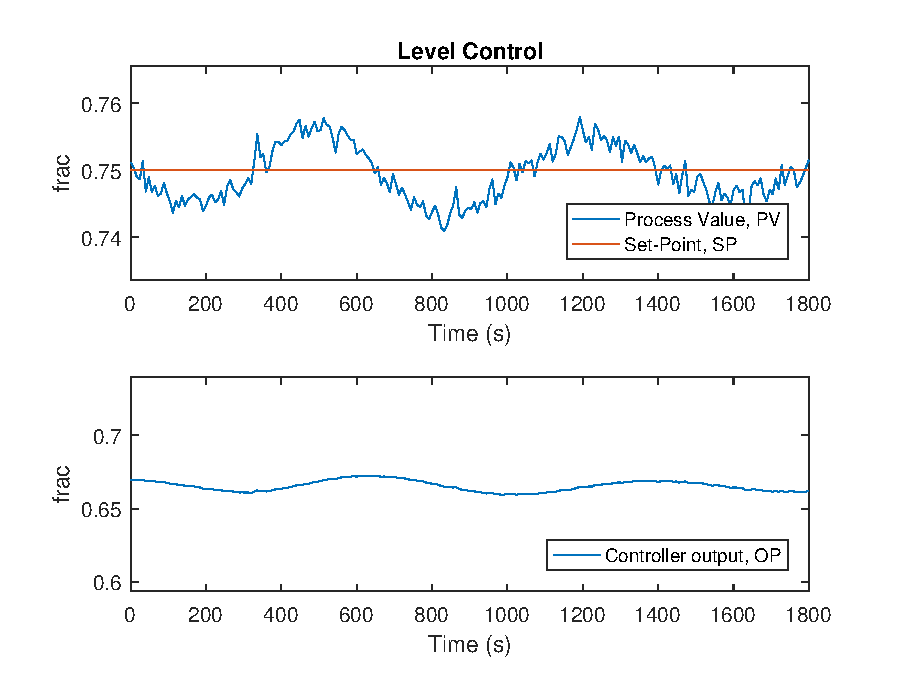
\includegraphics[width=0.7\textwidth]{fig/untuned/LIC0002_step1_untuned.eps}
	\caption{Response in \texttt{LIC0002} with step in the controller \texttt{LIC0001}}
	\label{fig:5a2}
\end{figure}
\begin{figure}[ht!]
	\centering
	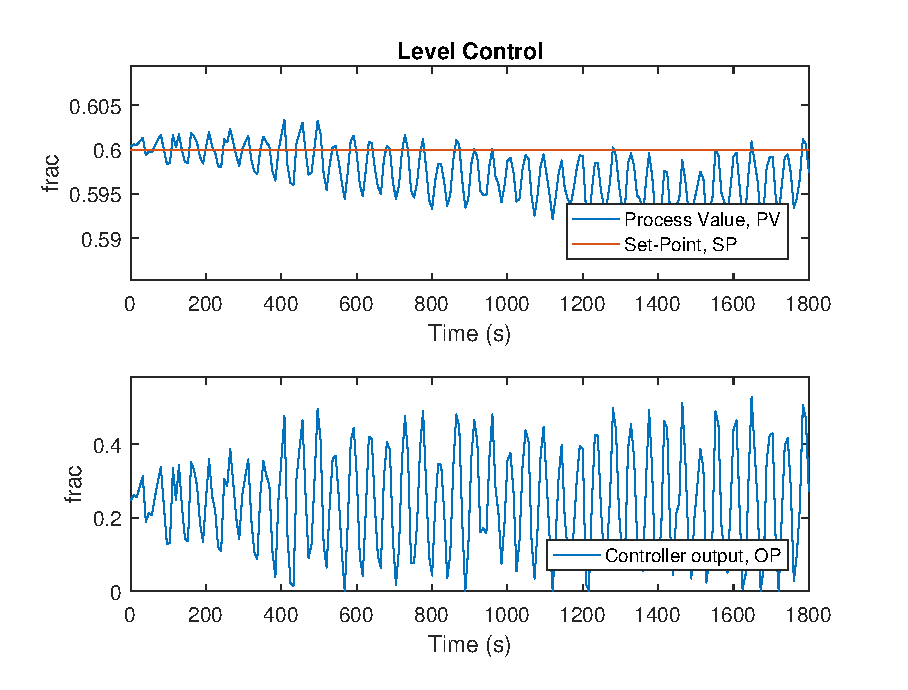
\includegraphics[width=0.7\textwidth]{fig/untuned/LIC0001_step2_untuned.eps}
	\caption{Response in \texttt{LIC0001} with step in the controller \texttt{LIC0002}}
	\label{fig:5a3}
\end{figure}
\begin{figure}[ht!]
	\centering
	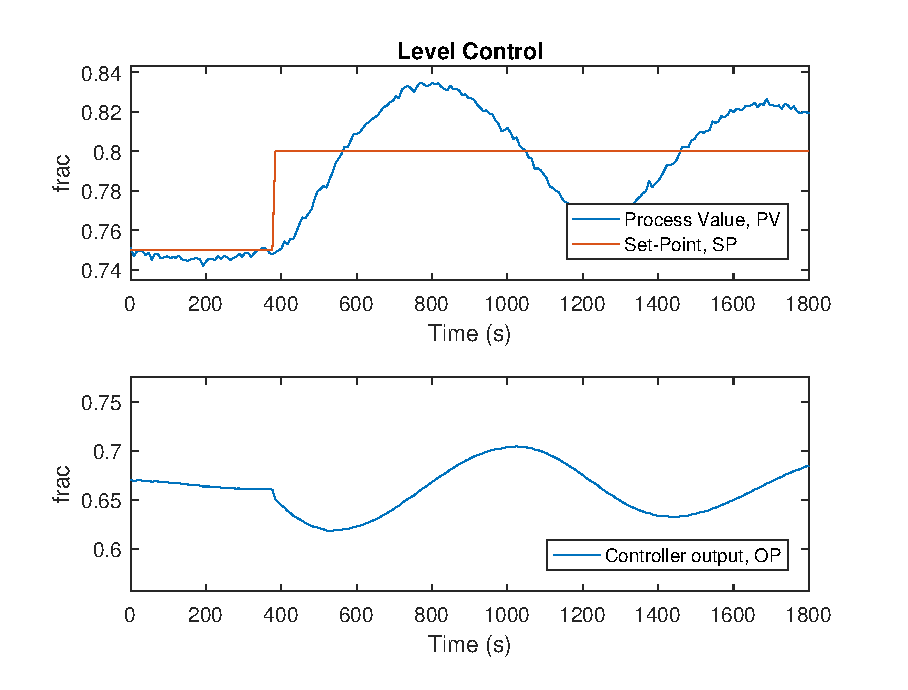
\includegraphics[width=0.7\textwidth]{fig/untuned/LIC0002_step2_untuned.eps}
	\caption{Response in \texttt{LIC0002} with step in the controller \texttt{LIC0002}}
	\label{fig:5a4}
\end{figure}

\begin{figure}[ht!]
	\centering
	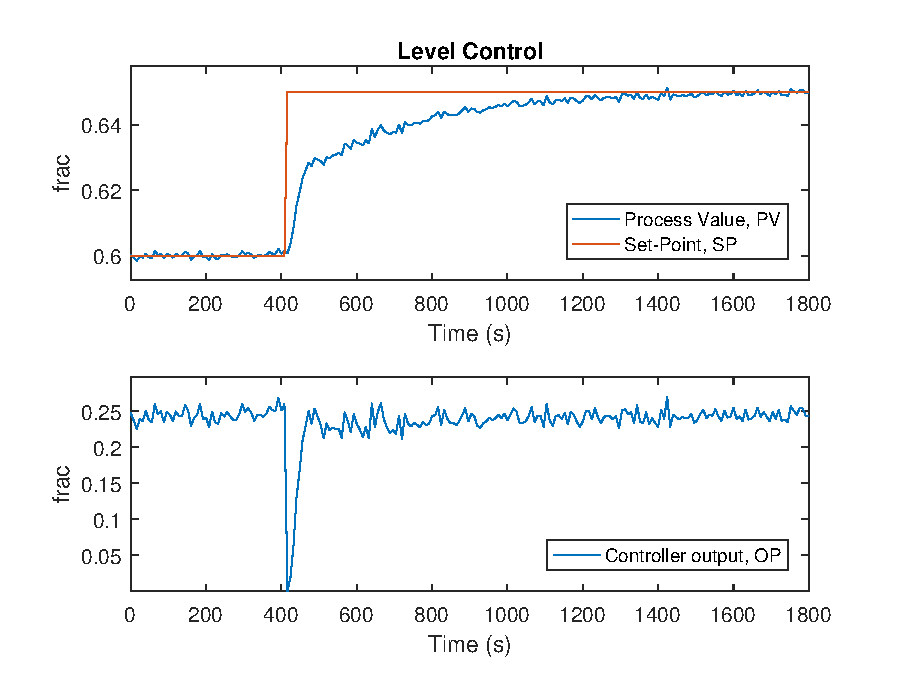
\includegraphics[width=0.8\textwidth]{fig/tuned/LIC0001_step1_tuned.eps}
	\caption{Tuned response in \texttt{LIC0001} with step in \texttt{LIC0001}}
	\label{fig:5b1}
\end{figure}
\begin{figure}[ht!]
	\centering
	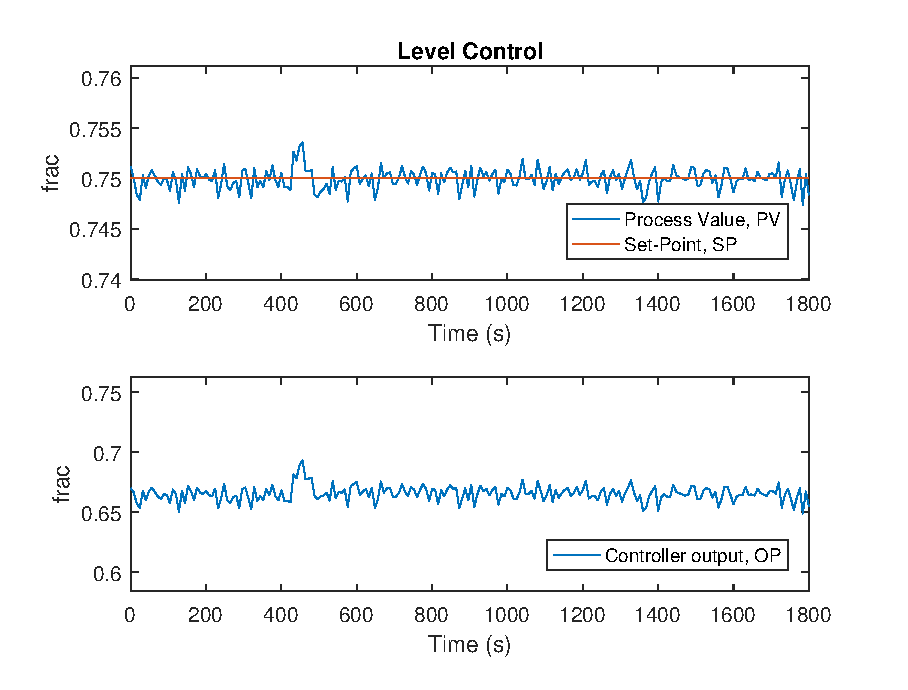
\includegraphics[width=0.8\textwidth]{fig/tuned/LIC0002_step1_tuned.eps}
	\caption{Tuned response in \texttt{LIC0002} with step in \texttt{LIC0001}}
	\label{fig:5b2}
\end{figure}
\begin{figure}[ht!]
	\centering
	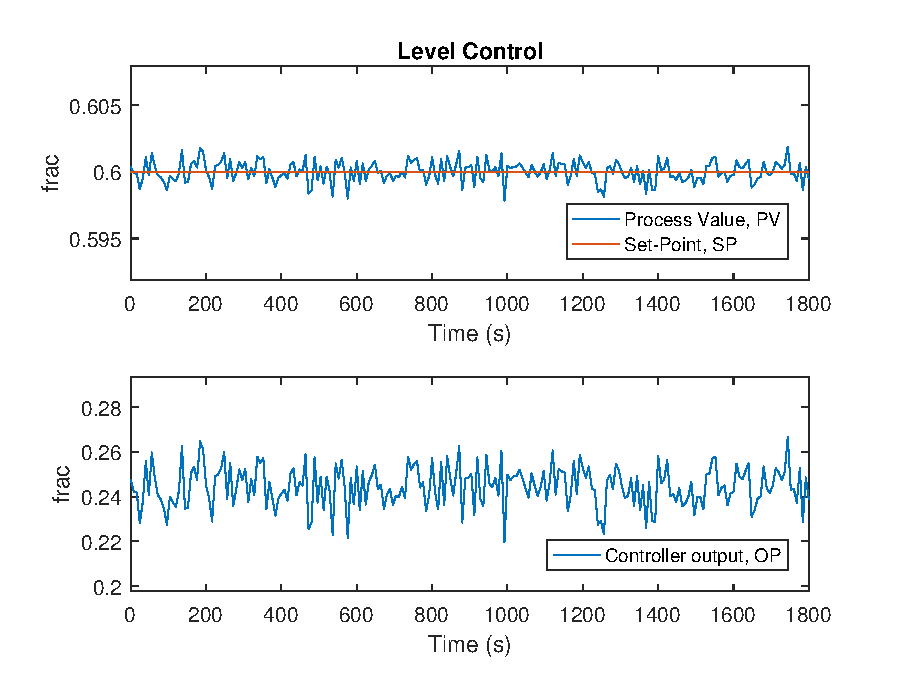
\includegraphics[width=0.8\textwidth]{fig/tuned/LIC0001_step2_tuned.eps}
	\caption{Tuned response in \texttt{LIC0001} with step in \texttt{LIC0002}}
	\label{fig:5b3}
\end{figure}
\begin{figure}[ht!]
	\centering
	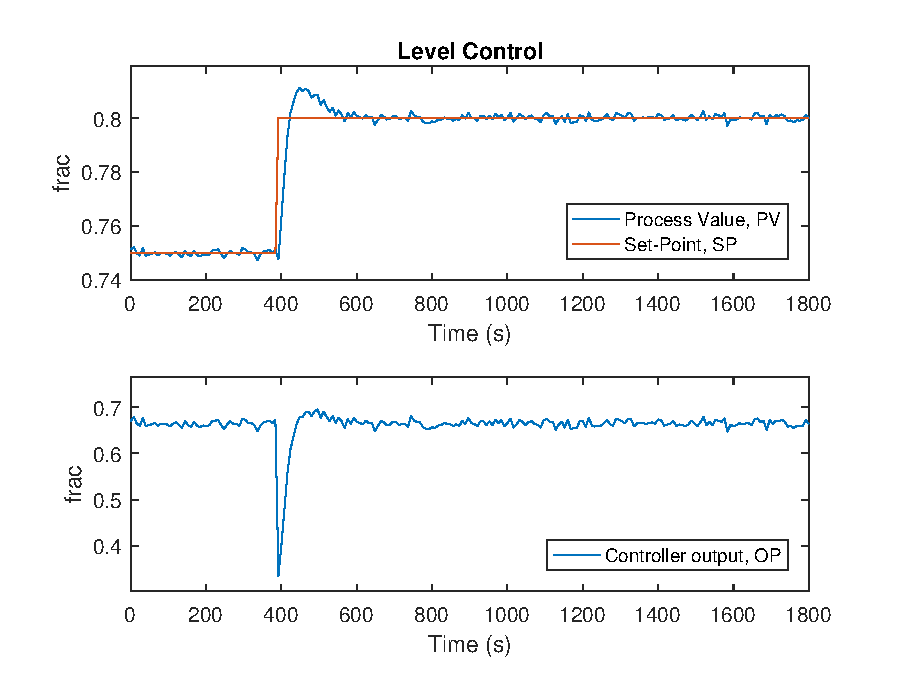
\includegraphics[width=0.8\textwidth]{fig/tuned/LIC0002_step2_tuned.eps}
	\caption{Tuned response in \texttt{LIC0002} with step in \texttt{LIC0002}}
	\label{fig:5b4}
\end{figure}


\end{document}